% !TeX root = main.tex

\newcommand{\ByronPortada}{%
  \begin{titlepage}
    \fontsize{12}{14}\selectfont
    \renewcommand{\arraystretch}{1.3}
    \centering
    {\Large\bfseries Universidad Técnica Estatal de Quevedo\par}
    \vspace{0.4cm}
    Facultad de Ciencias de la Computación\par
    Carrera de Software\par
    \vspace{1.2cm}
    {\Large\bfseries CLAB\par}
    \vspace{0.3cm}
    {\large Sistema distribuido de gestión de laboratorios\par}
    \vspace{0.8cm}
    \textbf{Proyecto Fin de Curso, entrega 1}\par
    Definición, requisitos y arquitectura base del sistema distribuido\par
    \vspace{0.8cm}
    TA-PFC-E1\par
    Aplicaciones Distribuidas (ISR-701)\par
    Séptimo nivel, paralelo A\par
    Periodo académico regular 2026-2027 SPA\par
    \vspace{0.8cm}
    \begin{tabular}{|p{0.43\textwidth}|p{0.43\textwidth}|}
      \hline
      \textbf{Integrante} & \textbf{Rol} \\ \hline
      Byron Daniel Loor Mendoza & Responsable de Documentación \\ \hline
      Roger Garcia & Arquitecto \\ \hline
      Juliana Emanuel Pino & Líder de Desarrollo \\ \hline
      Carlos Manotoa & Responsable de Calidad \\ \hline
    \end{tabular}
    \vspace{0.8cm}

    \textbf{Docente}\par
    Gleiston Cicerón Guerrero Ulloa\par
    \vspace{0.6cm}
    \textbf{Entrega prevista}\par
    29 de noviembre de 2026\par
    \vspace{0.6cm}
    \textbf{Repositorio del proyecto}\par
    \url{https://github.com/Danxxx777/clab-pfc-7a}\par
    \vfill
    Quevedo, Los Ríos, Ecuador\par
  \end{titlepage}
}

\newcommand{\ByronResumen}{%
  \section*{Resumen ejecutivo}
  CLAB es un proyecto universitario orientado a la gestión de los laboratorios
  informáticos de la Facultad de Ciencias de la Computación de la Universidad
  Técnica Estatal de Quevedo. El informe original describe reservas coordinadas
  por correo o mensajería, inventarios en hojas de cálculo, reportes verbales de
  fallas y dificultades para disponer de información consolidada sobre el uso
  de los espacios. Ese antecedente documenta una aplicación con Angular,
  Spring Boot y PostgreSQL y sirve como punto de partida para su evolución
  durante el Proyecto Fin de Curso de Aplicaciones Distribuidas
  \cite[pp.~4--5, 19--20]{clabAntecedente2026}.

  Los usuarios previstos son docentes, coordinadores de carrera, administradores
  de laboratorio y administradores del sistema. Los docentes consultarán la
  disponibilidad, gestionarán reservas y comunicarán fallas. La coordinación
  académica utilizará la agenda y los reportes para planificar el uso de los
  laboratorios. La administración de laboratorio mantendrá el catálogo y el
  inventario, mientras que la administración del sistema gestionará accesos,
  permisos y bloqueos institucionales.

  La arquitectura propuesta agrupa los módulos del legado en cuatro servicios
  por dominio, Identidad y Académico, Laboratorios y Recursos, Reservas y Agenda,
  e Información y Avisos. La distribución busca permitir despliegues
  independientes y aislar el procesamiento de reportes y notificaciones de la
  confirmación de reservas. Cada servicio tendrá almacenamiento de su propiedad.
  La agenda conservará una autoridad sobre la ocupación para evitar
  confirmaciones incompatibles. Estas decisiones se contrastarán con los
  requisitos de calidad y con el costo de introducir dependencias de red.

  El alcance académico se organiza en cuatro entregas. E1 establece los
  requisitos y la arquitectura y demuestra la comunicación entre dos procesos.
  E2 desarrollará las API y la contenerización. E3 abordará los datos y el
  procesamiento distribuido. E4 completará la integración, las pruebas y la
  observabilidad. El esqueleto actual permite consultar Laboratorios desde
  Reservas y observar un error cuando la dependencia está detenida.

  La validación combinará criterios funcionales, pruebas de concurrencia y
  mediciones de calidad. El diagnóstico del informe previo se conserva como
  antecedente. Su vinculación con el acta firmada o la grabación consentida
  exigida por E1 y la aprobación del alcance por el equipo siguen pendientes.
}

\newcommand{\ByronContexto}{%
  \section{Contexto y problema}
  \subsection{Organización y antecedente}
  El dominio del proyecto son los laboratorios informáticos de la Facultad de
  Ciencias de la Computación de la UTEQ. El informe original de CLAB identifica
  cuatro necesidades relacionadas, la coordinación de reservas, el inventario
  de equipos, el seguimiento de incidencias y la consulta de información para
  la planificación institucional \cite[pp.~4--5, 19--20]{clabAntecedente2026}.
  La versión desarrollada en semestres anteriores se consulta en el
  \href{https://github.com/Danxxx777/Clab--Sistema}{repositorio original de CLAB}.
  E1 parte de ese antecedente para definir la evolución
  distribuida y delimitar sus servicios.

  \subsection{Diagnóstico documentado}
  El informe previo describe reservas por correo electrónico y mensajería,
  con conflictos detectados al llegar al laboratorio. También reporta
  inventarios en archivos Excel sin una versión centralizada, fallas
  comunicadas verbalmente y falta de información estructurada para las
  decisiones de mantenimiento e inversión
  \cite[pp.~19--20]{clabAntecedente2026}.

  Como consecuencias, el documento señala pérdida de tiempo de clase,
  planificación con equipos fuera de servicio, reportes duplicados y
  mantenimiento reactivo. El intervalo de consulta de disponibilidad se
  describe cualitativamente como horas o días. Esa afirmación no aporta una
  muestra de tiempos ni un registro de mediciones. Para cuantificar el impacto
  se requiere conservar la fecha de cada solicitud y confirmación, la cantidad
  de conflictos y los tiempos de atención de incidencias. Esas mediciones
  siguen pendientes para la evaluación de E1.

  \subsection{Interesados identificados en el antecedente}
  Los perfiles y sus expectativas se obtienen de los requisitos y casos de uso
  del informe original \cite[pp.~14--15, 20, 25--32]{clabAntecedente2026}.
  \begin{description}
    \item[Docentes.] Consultar la agenda, gestionar sus reservas y registrar
    fallas de los equipos utilizados en las clases.
    \item[Coordinación de carrera.] Planificar el uso académico de los
    laboratorios, resolver conflictos y consultar reportes por carrera y periodo.
    \item[Administración de laboratorio.] Mantener el inventario y el estado
    de los recursos, atender incidencias y registrar asistencia.
    \item[Administración del sistema.] Gestionar usuarios y permisos,
    registrar bloqueos institucionales y consultar la auditoría.
  \end{description}

  \subsection{Respaldo del levantamiento}
  El Anexo A del informe contiene el cuestionario para autoridades, docentes y
  administradores. El Anexo B incluye una fotografía identificada como
  evidencia de entrevistas \cite[pp.~45--47]{clabAntecedente2026}. La copia
  recibida se conserva sin modificaciones en
  \path{evidencias/antecedentes/CLAB-informe-original-2026.pdf}.
  La identificación del entrevistado, su cargo, la fecha y el acta firmada o
  el audio con consentimiento siguen pendientes de incorporación. Por ello,
  la trazabilidad inicial de las historias remite a los requisitos del informe
  previo y deberá completarse con el registro primario del levantamiento.
}

\newcommand{\ByronObjetivos}{%
  \section{Objetivos propuestos}
  \subsection{Objetivo general}
  Evolucionar CLAB hacia una aplicación distribuida para la gestión de
  laboratorios informáticos de la UTEQ durante las cuatro entregas del PFC,
  conservando la integridad de la agenda y evaluando su comportamiento
  mediante requisitos funcionales, de rendimiento y de seguridad verificables.

  \subsection{Objetivos específicos e indicadores}
  \begin{description}
    \item[OE-01] Consolidar el alcance funcional y su trazabilidad durante E1.
    \textbf{Indicador propuesto:} dieciséis historias con criterios de
    aceptación, al menos seis requisitos no funcionales cuantificados y
    vinculación de cada historia con el levantamiento primario.

    \item[OE-02] Implementar los cuatro servicios por dominio propuestos en
    ADR-001 mediante incrementos de E2 a E4.
    \textbf{Indicador propuesto:} cuatro servicios desplegables de forma
    independiente, con API documentada y propiedad explícita de sus datos.

    \item[OE-03] Evaluar la respuesta de las consultas de disponibilidad con
    el escenario definido en RNF-01.
    \textbf{Indicador propuesto:} al menos el 95\,\% de respuestas correctas
    en menos de dos segundos durante diez minutos de carga estable con
    cincuenta usuarios virtuales concurrentes.

    \item[OE-04] Verificar la integridad y la autorización de las operaciones
    de agenda al final del periodo.
    \textbf{Indicador propuesto:} cero confirmaciones superpuestas para un
    mismo laboratorio e intervalo y cero operaciones protegidas ejecutadas
    sin permiso válido en el conjunto de pruebas documentado.

    \item[OE-05] Incorporar pruebas y observabilidad en la entrega E4.
    \textbf{Indicador propuesto:} una canalización CI/CD que ejecute las
    pruebas unitarias y de integración, un informe de pruebas de carga y
    evidencia de métricas, logs y trazas de los servicios evaluados.
  \end{description}
}

\newcommand{\ByronHistoriasUsuario}{%
  \subsection{Requisitos funcionales como historias de usuario}
  Las siguientes dieciséis historias adaptan los RF-01 a RF-16 de la Tabla 4
  del informe original \cite[pp.~14--15]{clabAntecedente2026}. Son una propuesta
  de alcance para la versión distribuida. Su aceptación por el equipo y su
  vinculación con el registro primario de entrevistas siguen pendientes.

  \begin{description}
    \item[HU-01] \textbf{Autenticación, origen RF-01.}
    Como usuario institucional, quiero iniciar sesión con mis credenciales
    para acceder a las funciones autorizadas.
    \textbf{Criterio:} las credenciales válidas permiten obtener una sesión
    identificada y las credenciales inválidas impiden acceder a las funciones
    protegidas.

    \item[HU-02] \textbf{Permisos por rol, origen RF-02.}
    Como administrador del sistema, quiero asignar roles y permisos para
    controlar el acceso a las funciones.
    \textbf{Criterio:} un usuario autorizado ejecuta la operación asignada a su
    rol; una cuenta sin ese permiso recibe una denegación y la operación queda
    sin ejecutar.

    \item[HU-03] \textbf{Catálogo de laboratorios, origen RF-03.}
    Como administrador de laboratorio, quiero gestionar sus datos y recursos
    para mantener disponible un catálogo actualizado.
    \textbf{Criterio:} al registrar o modificar un laboratorio, sus datos de
    ubicación, capacidad y equipamiento pueden consultarse posteriormente.

    \item[HU-04] \textbf{Disponibilidad, origen RF-04.}
    Como docente, quiero consultar la disponibilidad por laboratorio, fecha y
    horario para planificar una actividad práctica.
    \textbf{Criterio:} una franja ocupada por una reserva o un bloqueo vigente
    se muestra con ese estado en la agenda consultada.

    \item[HU-05] \textbf{Gestión de reservas, origen RF-05.}
    Como docente, quiero registrar, consultar y cancelar mis reservas para
    gestionar el uso del laboratorio.
    \textbf{Criterio:} una solicitud válida aparece en el calendario y en la
    consulta de reservas propias. Al cancelar una reserva propia pendiente o
    confirmada, queda registrado el motivo y se libera su ocupación. El caso
    de uso CU-02 documenta esta cancelación
    \cite[p.~26]{clabAntecedente2026}.

    \item[HU-06] \textbf{Conflictos de horario, origen RF-06.}
    Como docente, quiero conocer los conflictos y las alternativas disponibles
    para evitar reservas incompatibles.
    \textbf{Criterio:} si el laboratorio está ocupado en el intervalo
    solicitado, se rechaza la confirmación y se muestran las alternativas
    disponibles. Si no existen alternativas, se informa ese resultado.

    \item[HU-07] \textbf{Inventario, origen RF-07.}
    Como administrador de laboratorio, quiero registrar los equipos con su
    número de serie, tipo, marca y modelo para identificarlos en el inventario.
    \textbf{Criterio:} el equipo registrado puede consultarse y el sistema
    rechaza otro registro con el mismo número de serie.

    \item[HU-08] \textbf{Estado de equipos, origen RF-08.}
    Como administrador de laboratorio, quiero actualizar el estado operativo
    de los equipos para conocer su disponibilidad técnica.
    \textbf{Criterio:} el cambio a operativo, mantenimiento o fuera de
    servicio se conserva con la fecha y el usuario responsable.

    \item[HU-09] \textbf{Reporte de fallas, origen RF-09.}
    Como docente, quiero reportar una falla asociada al laboratorio y al equipo
    para que su responsable pueda atenderla.
    \textbf{Criterio:} un reporte con los datos requeridos queda registrado
    y puede consultarse desde la administración del laboratorio correspondiente.

    \item[HU-10] \textbf{Seguimiento de fallas, origen RF-10.}
    Como administrador de laboratorio, quiero actualizar el estado de una
    incidencia para dar seguimiento a su resolución.
    \textbf{Criterio:} el reporte conserva los cambios entre abierta, en
    atención, resuelta y cerrada, junto con su historial.

    \item[HU-11] \textbf{Bloqueos institucionales, origen RF-11.}
    Como administrador del sistema, quiero registrar bloqueos por
    mantenimiento o eventos para impedir nuevas reservas en esos intervalos.
    \textbf{Criterio:} después de confirmar el bloqueo en la agenda, el
    intervalo afectado deja de ofrecerse como disponible.

    \item[HU-12] \textbf{Asistencia, origen RF-12.}
    Como administrador de laboratorio, quiero registrar la asistencia a una
    reserva confirmada para documentar el uso del espacio.
    \textbf{Criterio:} cada registro de presencia o ausencia queda vinculado
    con el participante y la reserva correspondiente.

    \item[HU-13] \textbf{Reportes de uso, origen RF-13.}
    Como coordinador de carrera, quiero consultar reportes por carrera y
    periodo académico para apoyar la planificación de laboratorios.
    \textbf{Criterio:} el reporte muestra los datos correspondientes a los
    filtros seleccionados y permite su visualización o exportación.

    \item[HU-14] \textbf{Auditoría, origen RF-14.}
    Como administrador del sistema, quiero consultar las acciones registradas
    para identificar quién realizó cada operación.
    \textbf{Criterio:} las operaciones auditadas incluyen usuario, fecha y
    operación, y pueden recuperarse desde la consulta de auditoría.

    \item[HU-15] \textbf{Avisos internos, origen RF-15.}
    Como usuario afectado por una reserva o incidencia, quiero recibir sus
    notificaciones para conocer los cambios relacionados.
    \textbf{Criterio:} el destinatario puede consultar dentro del sistema
    el aviso de una confirmación, un conflicto o un cambio registrado.

    \item[HU-16] \textbf{Información académica, origen RF-16.}
    Como coordinador de carrera, quiero gestionar carreras, asignaturas,
    horarios y periodos para vincularlos con las reservas académicas.
    \textbf{Criterio:} una reserva permite asociar y consultar los datos
    académicos registrados que le corresponden.
  \end{description}
}


\newcommand{\ByronTablaAportes}{%
  \section{Tabla de aportes}

  El corte de esta revisión es el 21 de noviembre de 2026. Los enlaces
  corresponden a commits presentes en la rama \texttt{main}. Las actividades
  registradas con asistencia de IA se detallan en la bitácora y en las
  declaraciones de sus responsables.

  \begin{table*}[!t]
  \caption{Aportes registrados y enlaces de seguimiento.}
  \label{tab:aportes}
  \centering
  \small
  \setlength{\tabcolsep}{4pt}
  \renewcommand{\arraystretch}{1.1}
  \begin{tabular}{|>{\raggedright\arraybackslash}p{0.23\textwidth}|>{\raggedright\arraybackslash}p{0.48\textwidth}|>{\raggedright\arraybackslash}p{0.21\textwidth}|}
    \hline
    \textbf{Integrante o cuenta} & \textbf{Trabajo registrado} &
    \textbf{Commits e issue} \\ \hline

    Byron Daniel Loor Mendoza\par\texttt{Danxxx777} &
    Organización inicial del esqueleto; conservación del informe antecedente;
    portada, resumen, contexto, interesados, objetivos y dieciséis historias
    de usuario; integración documental de los aportes disponibles.
    La asistencia de Codex está registrada en \texttt{BITACORA.md}. &
    \href{https://github.com/Danxxx777/clab-pfc-7a/commit/f57fa6b}{\texttt{f57fa6b}}\par
    \href{https://github.com/Danxxx777/clab-pfc-7a/commit/10f727a}{\texttt{10f727a}}\par
    \href{https://github.com/Danxxx777/clab-pfc-7a/commit/065e173}{\texttt{065e173}}\par
    \href{https://github.com/Danxxx777/clab-pfc-7a/commit/20be179}{\texttt{20be179}}\par
    \href{https://github.com/Danxxx777/clab-pfc-7a/commit/1fb56f2}{\texttt{1fb56f2}}\par
    \href{https://github.com/Danxxx777/clab-pfc-7a/issues/1}{Issue 1}
    \\ \hline

    Roger Garcia\par\texttt{Esteiben} &
    Propuesta de arquitectura distribuida, ADR-001 y diagramas C4 editables.
    El registro conserva el estado propuesto de las decisiones. &
    \href{https://github.com/Danxxx777/clab-pfc-7a/commit/d65150e}{\texttt{d65150e}}\par
    \href{https://github.com/Danxxx777/clab-pfc-7a/commit/c4d79ac}{\texttt{c4d79ac}}\par
    \href{https://github.com/Danxxx777/clab-pfc-7a/issues/2}{Issue 2}
    \\ \hline

    Juliana Emanuel Pino\par\texttt{JulianaEmanuel} &
    Actualización del runtime a Java 25 y borradores de los diagramas C4
    y del análisis CAP y PACELC. &
    \href{https://github.com/Danxxx777/clab-pfc-7a/commit/bbbf3dd}{\texttt{bbbf3dd}}\par
    \href{https://github.com/Danxxx777/clab-pfc-7a/commit/62276a6}{\texttt{62276a6}}\par
    \href{https://github.com/Danxxx777/clab-pfc-7a/commit/85e7c67}{\texttt{85e7c67}}\par
    \href{https://github.com/Danxxx777/clab-pfc-7a/issues/3}{Issue 3}
    \\ \hline

    Carlos Manotoa\par\texttt{CarlosManotoa007} &
    Bibliografía, comparación de tres estudios, siete requisitos no
    funcionales, cinco riesgos técnicos, tres capturas de ejecución y
    declaración individual de IA. &
    \href{https://github.com/Danxxx777/clab-pfc-7a/commit/8cf8f12}{\texttt{8cf8f12}}\par
    \href{https://github.com/Danxxx777/clab-pfc-7a/commit/c8d6659}{\texttt{c8d6659}}\par
    \href{https://github.com/Danxxx777/clab-pfc-7a/commit/75bd4d6}{\texttt{75bd4d6}}\par
    \href{https://github.com/Danxxx777/clab-pfc-7a/commit/d25d245}{\texttt{d25d245}}\par
    \href{https://github.com/Danxxx777/clab-pfc-7a/commit/3bce9ba}{\texttt{3bce9ba}}\par
    \href{https://github.com/Danxxx777/clab-pfc-7a/commit/b212d70}{\texttt{b212d70}}\par
    \href{https://github.com/Danxxx777/clab-pfc-7a/issues/4}{Issue 4}
    \\ \hline
  \end{tabular}
  \end{table*}

  \paragraph{Vinculación con issues.}
  Las issues 1 a 4 se crearon el 21 de noviembre de 2026 y se asignaron a
  las cuentas indicadas. Registran el estado de los aportes y los pendientes
  de cada rol después de los commits enlazados. Permanecen abiertas para
  completar las verificaciones y evidencias de cierre. Su incorporación
  al tablero de GitHub Projects corresponde al plan del equipo.
}

\newcommand{\ByronDeclaracionIntegracion}{%
  \paragraph{Byron Daniel Loor Mendoza, Responsable de Documentación.}
  Se utilizó OpenAI Codex (familia de modelos GPT-6) para organizar los
  antecedentes y el documento, preparar borradores a partir del informe
  original e integrar los aportes y archivos del repositorio. La revisión
  comprendió ortografía y puntuación, correspondencia con las fuentes citadas,
  enlaces a commits, compilación con pdfLaTeX y Biber y presentación del PDF.
  La validación de las propuestas con el levantamiento primario y su aprobación
  por el equipo siguen pendientes.
}

\newcommand{\ByronDeclaracionesRegistradas}{%
  \paragraph{Arquitectura, cuenta Esteiben.}
  ADR-001 y la justificación registran asistencia de OpenAI, modelo GPT-6.1 Sol,
  en la preparación de la propuesta a partir del documento previo y del código
  consultado. Los registros distinguen los dos procesos mínimos de E1 de los
  cuatro servicios propuestos. La integración comprobó la presencia de los
  diagramas editables, sus figuras y las citas del documento.

  \paragraph{Desarrollo y CAP/PACELC, cuenta JulianaEmanuel.}
  El archivo \path{docs/arquitectura/cap-pacelc.tex} registra asistencia de
  OpenAI Codex para preparar el borrador a partir de ADR-001 y del controlador
  de E1. Ese registro no consigna la versión concreta del modelo. La
  verificación técnica de esta integración comprobó la compilación de ese
  apartado y la resolución de sus citas. La confirmación de la versión usada
  y de la revisión personal corresponde a su responsable.
}

\newcommand{\ByronEvidenciasEsqueleto}{%
  \section{Capturas de ejecución del esqueleto}
  Las tres capturas fueron incorporadas por la cuenta
  \texttt{CarlosManotoa007} en el commit
  \href{https://github.com/Danxxx777/clab-pfc-7a/commit/3bce9ba}{\texttt{3bce9ba}}.
  Muestran el usuario \texttt{carlos}, el equipo \texttt{cachyos-x8664} y
  la fecha del sistema, 20 de noviembre de 2026, con zona horaria UTC-5.

  \begin{figure*}[!t]
    \centering
    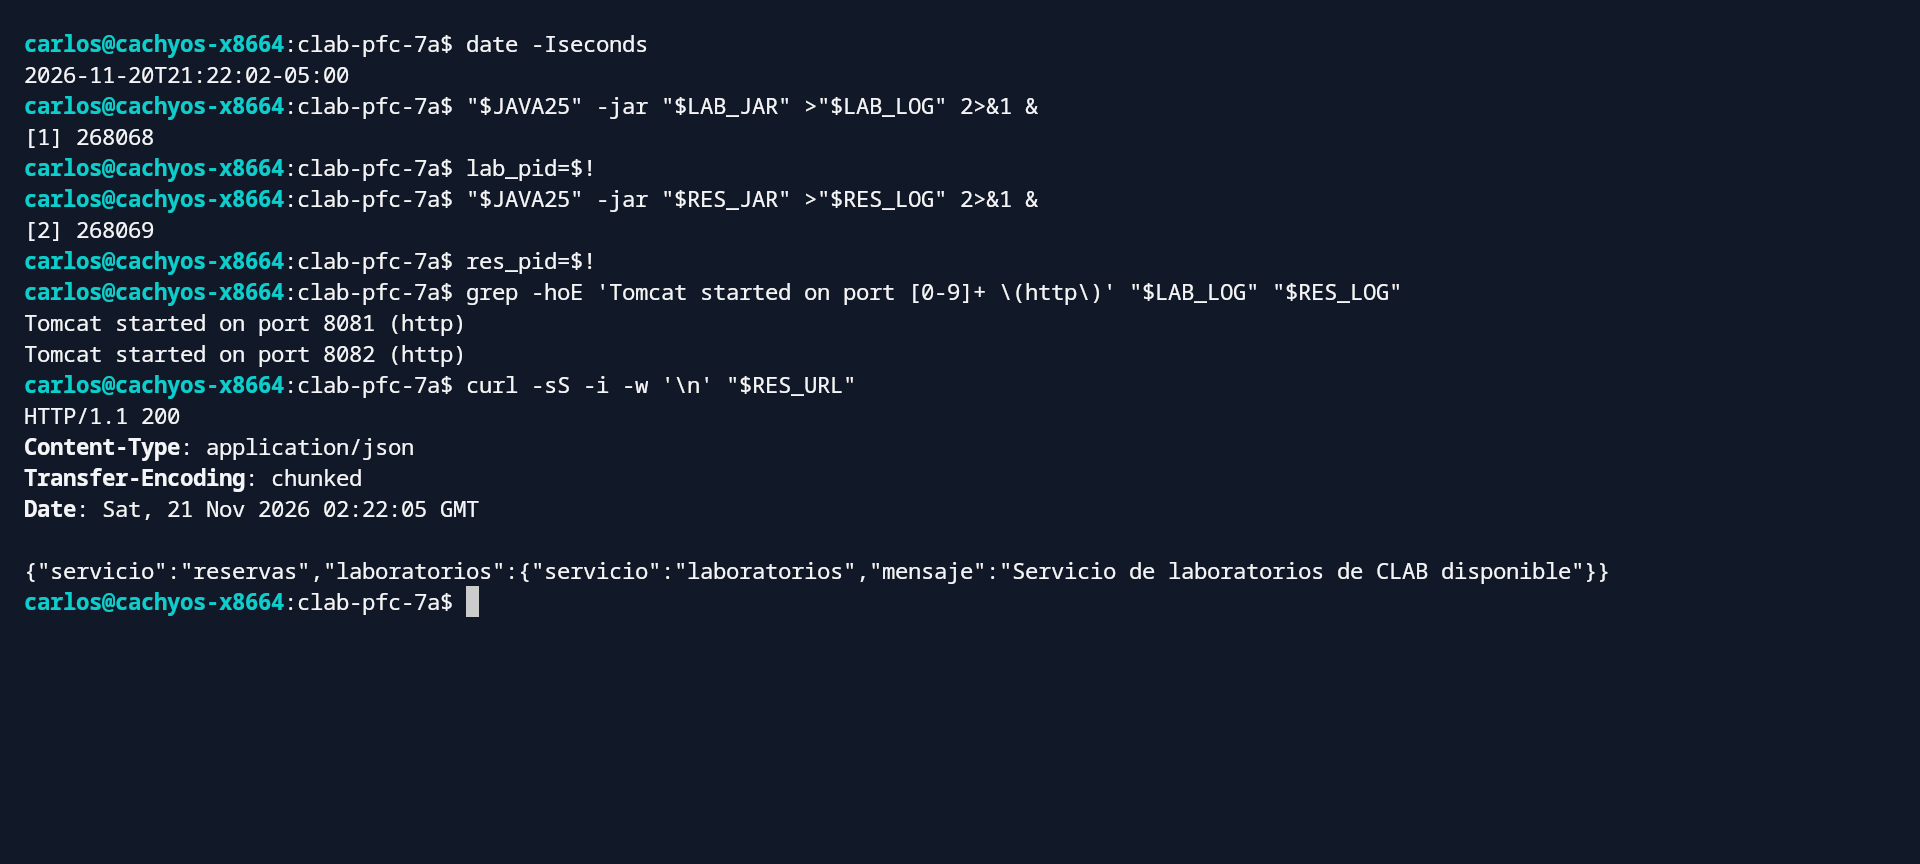
\includegraphics[width=\textwidth]{../evidencias/Laboratorio.png}
    \caption{Arranque de los procesos en los puertos 8081 y 8082 y respuesta
    HTTP 200 de Reservas con el mensaje recibido de Laboratorios.}
  \end{figure*}

  \begin{figure*}[!t]
    \centering
    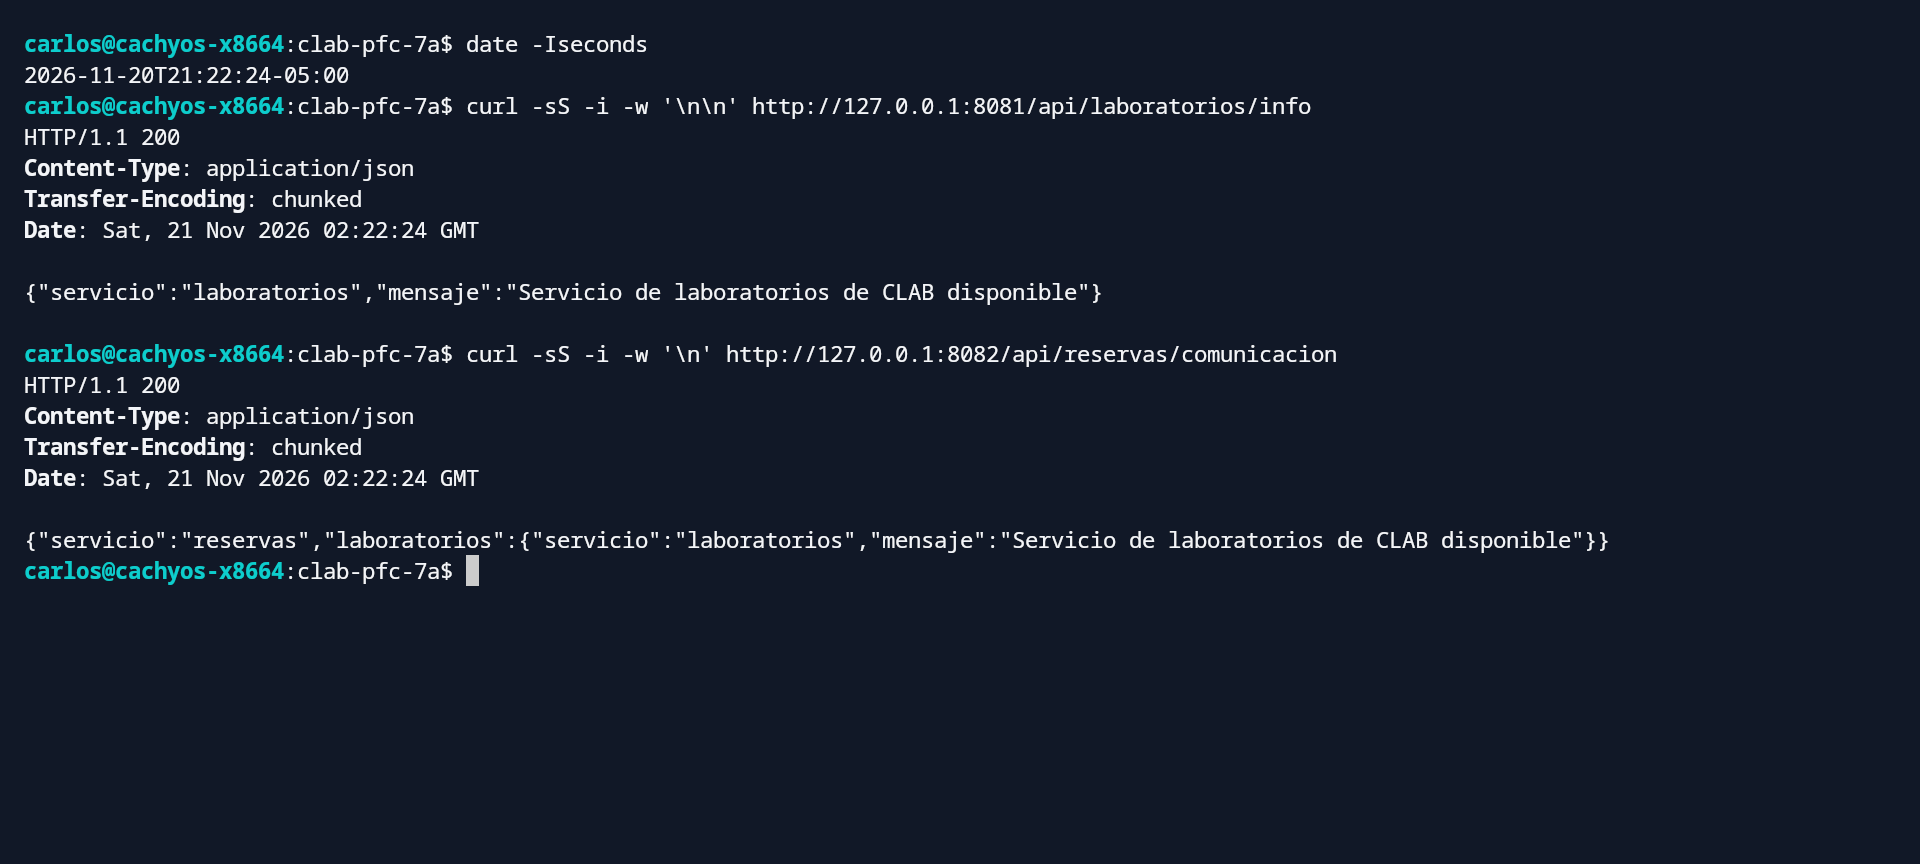
\includegraphics[width=\textwidth]{../evidencias/Consultas.png}
    \caption{Consultas a Laboratorios y Reservas con respuestas HTTP 200 y
    contenido JSON.}
  \end{figure*}

  \begin{figure*}[!t]
    \centering
    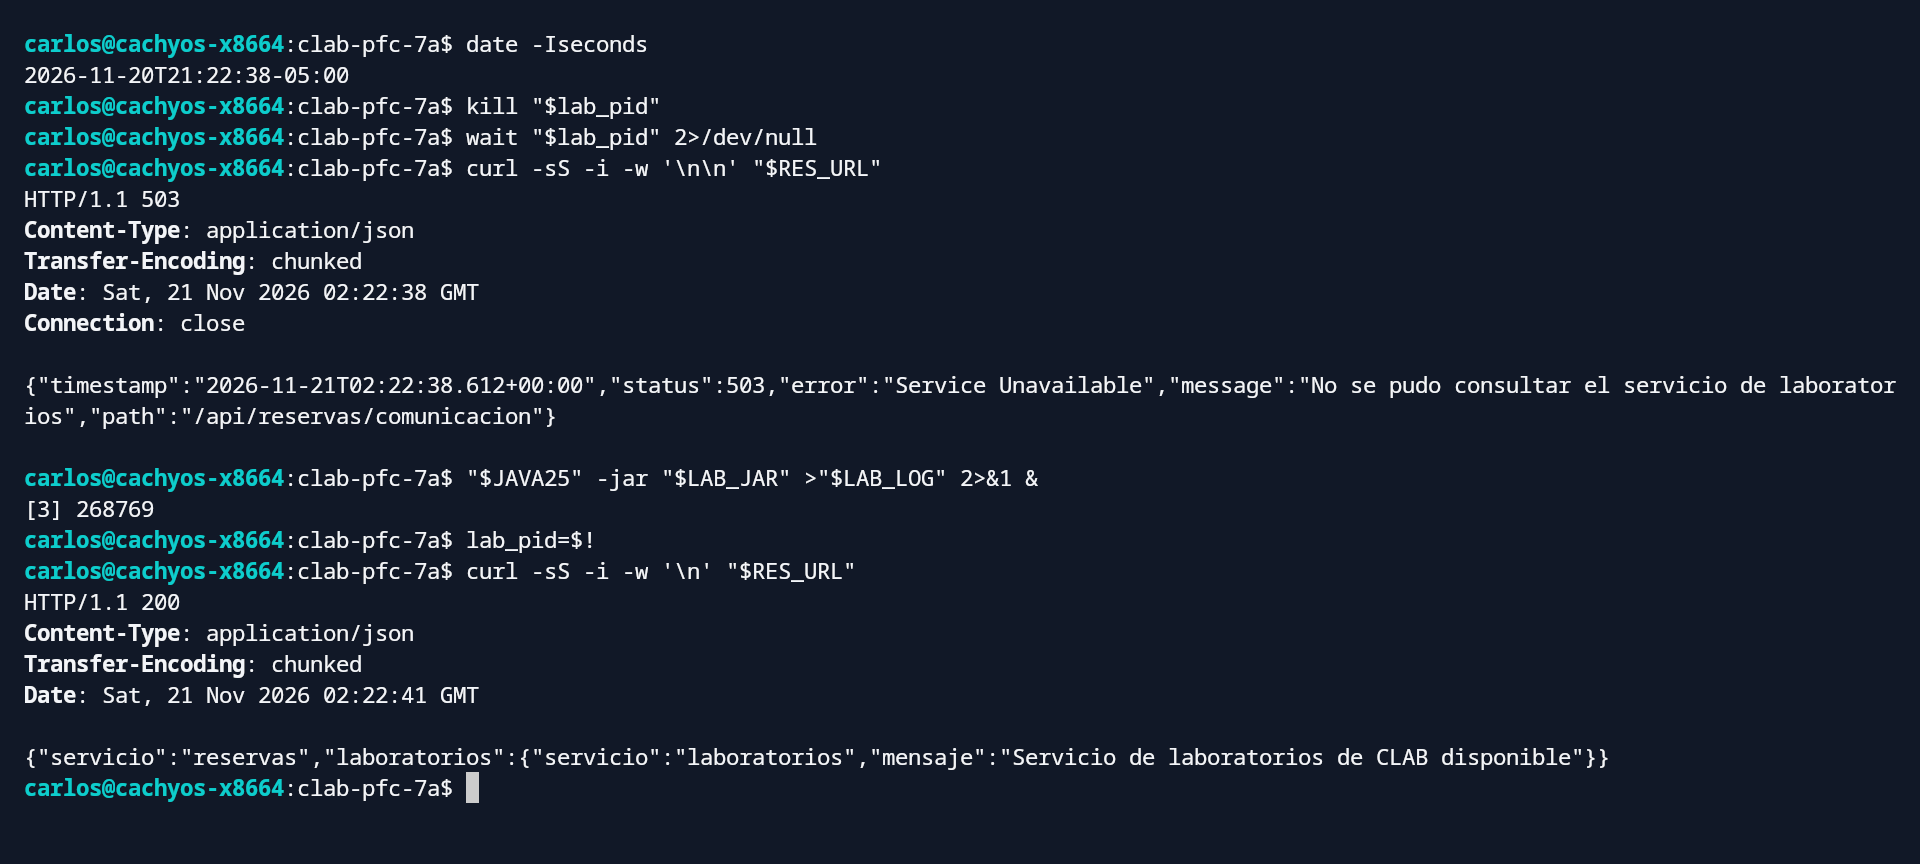
\includegraphics[width=\textwidth]{../evidencias/Reservas.png}
    \caption{Respuesta HTTP 503 al detener Laboratorios y nueva respuesta
    HTTP 200 tras volver a iniciar ese proceso.}
  \end{figure*}
}
